\documentclass{beamer}
\usetheme{Hannover}
\setbeamersize{sidebar width left=0pt}
\usepackage[T1, T2A]{fontenc}
\usepackage[utf8]{inputenc}
\usepackage[russian]{babel}
\usepackage{hyperref}
\usepackage{graphicx}
\graphicspath{ {../Images/} }

\author{Григорий Матюхин}
\date{\today}
\title{Лабораторная работа \textnumero16.}
\subtitle{Программный RAID}

\begin{document}
\begin{frame}[plain]
	\titlepage
\end{frame}
\section{Цель работы}
\begin{frame}[plain]
	\frametitle{Цель работы}
	Освоить работу с RAID-массивами при помощи утилиты \texttt{mdadm}.
\end{frame}

\subsection{Создание RAID-диска}
\begin{enumerate}
	\begin{frame}[plain]
		\frametitle{Создание RAID-диска}
		\item Запустите виртуальную машину. Получите полномочия администратора:
		\item Проверьте наличие созданных вами ранее дополнительных дисков:
		\\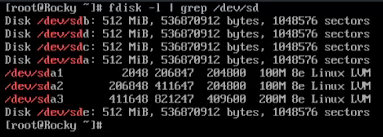
\includegraphics{1.png}
	\end{frame}
	\begin{frame}[plain]
		\item Создайте на каждом из дисков раздел:
		\\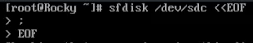
\includegraphics{2.png}
	\end{frame}
	\begin{frame}[plain]
		\item Просмотрите, какие типы партиций, относящиеся к RAID, можно задать:
		\\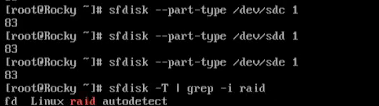
\includegraphics{3.png}
		\\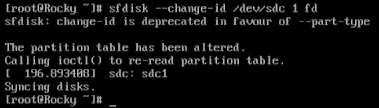
\includegraphics{4.png}
	\end{frame}
	\begin{frame}[plain]
		\item Просмотрите состояние дисков:
		\\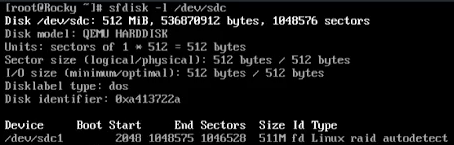
\includegraphics{5.png}
	\end{frame}
	\begin{frame}[plain]
		\item При помощи утилиты \texttt{mdadm} создайте массив RAID 1 из двух дисков:
		\\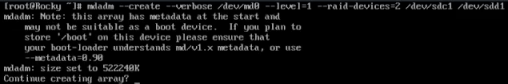
\includegraphics{6.png}
	\end{frame}
	\begin{frame}[plain]
		\item Проверьте состояние массива RAID:
		\\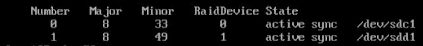
\includegraphics{7.png}
	\end{frame}
	\begin{frame}[plain]
		\item Создайте файловую систему на RAID:
		\item Подмонтируйте RAID:
		%\\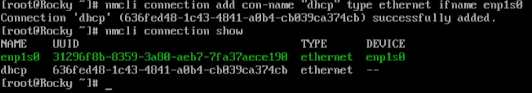
\includegraphics{8.png}
		\item Для автомонтирования добавьте запись в \texttt{/etc/fstab}:
		%\\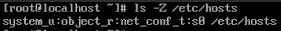
\includegraphics{9.png}
		\item Сымитируйте сбой одного из дисков:
		\item Удалите сбойный диск:
		\item Замените диск в массиве:
		\\
\includegraphics{10.png}
	\end{frame}
	\begin{frame}[plain]
		\item Посмотрите состояние массива:
		\\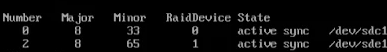
\includegraphics{11.png}
	\end{frame}
	\begin{frame}[plain]
		\item Удалите массив и очистите метаданные:
		\\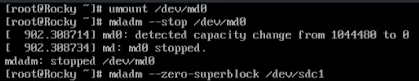
\includegraphics{12.png}
	\end{frame}
\end{enumerate}

\subsection{RAID-массив с горячим резервом (hotspare)}
\begin{enumerate}
	\begin{frame}[plain]
		\frametitle{RAID-массив с горячим резервом (hotspare)}
		\item Создайте массив RAID 1 из двух дисков:
		\\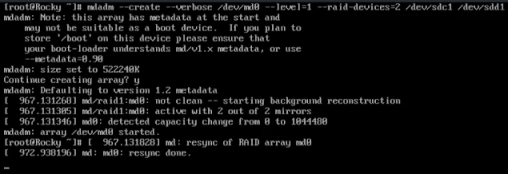
\includegraphics{13.png}
	\end{frame}
	\begin{frame}[plain]
		\item Добавьте третий диск:
		\\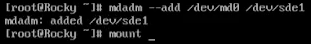
\includegraphics{14.png}
	\end{frame}
	\begin{frame}[plain]
		\item Подмонтируйте \texttt{/dev/md0}:
		\item Проверьте состояние массива:
		\\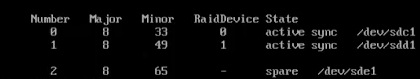
\includegraphics{15.png}
	\end{frame}
	\begin{frame}[plain]
		\item Сымитируйте сбой одного из дисков:
		\\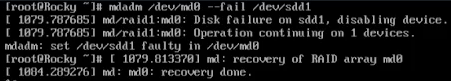
\includegraphics{16.png}
	\end{frame}
	\begin{frame}[plain]
		\item Проверьте состояние массива:
		\\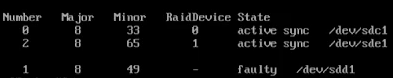
\includegraphics{17.png}
		\item Удалите массив и очистите метаданные:
	\end{frame}
\end{enumerate}

\subsection{Преобразование массива RAID 1 в RAID 5}
\begin{enumerate}
	\begin{frame}[plain]
		\frametitle{Преобразование массива RAID 1 в RAID 5}
		\item Создайте массив RAID 1 из двух дисков:
		\\
\includegraphics{18.png}
	\end{frame}
	\begin{frame}[plain]
		\item Добавьте третий диск:
		\\
\includegraphics{19.png}
	\end{frame}
	\begin{frame}[plain]
		\item Подмонтируйте \texttt{/dev/md0}:
		\item Проверьте состояние массива:
		\\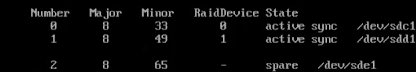
\includegraphics{20.png}
	\end{frame}
	\begin{frame}[plain]
		\item Измените тип массива RAID:
		\\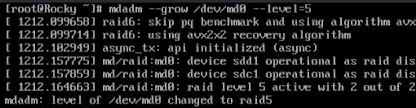
\includegraphics{21.png}
	\end{frame}
	\begin{frame}[plain]
		\item Проверьте состояние массива:
		\\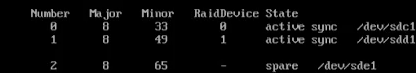
\includegraphics{22.png}
	\end{frame}
	\begin{frame}[plain]
		\item Измените количество дисков в массиве RAID 5:
		\\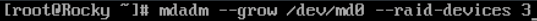
\includegraphics{23.png}
	\end{frame}
	\begin{frame}[plain]
		\item Проверьте состояние массива:
		\\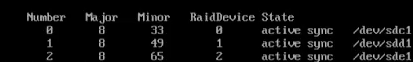
\includegraphics{24.png}
		\item Удалите массив и очистите метаданные:
		\item Закомментируйте запись в \texttt{/etc/fstab}:
	\end{frame}
\end{enumerate}

\section{Вывод}
\begin{frame}[plain]
	\frametitle{Вывод}
	В ходе выполнения данной работы я освоил работу с RAID-массивами при помощи утилиты \texttt{mdadm}.
\end{frame}

\end{document}
